% Document
\documentclass[fontsize=8pt,paper=a4,paper=landscape,DIV=calc,]{scrartcl}
\usepackage[T1]{fontenc}
\usepackage{noto}
\usepackage[nswissgerman,english]{babel}
\renewcommand{\familydefault}{\sfdefault}

% Format
\usepackage[top=5mm,bottom=1mm,left=5mm,right=5mm,includehead]{geometry}
\setlength{\headheight}{\baselineskip}
\setlength{\headsep}{0mm}

\usepackage{multicol}
\setlength{\columnsep}{2mm}
\setlength{\columnseprule}{0.1pt}

% Color
\usepackage[svgnames]{xcolor}

% Math
\usepackage{amsmath}
\usepackage{amssymb}
\usepackage{amsfonts}
\newcommand*{\eq}{=}

%% Venn Diagrams
\usepackage{venndiagram}

%% Trees
%%% https://tex.stackexchange.com/a/425271
\usepackage{forest}
\forestset{
    ptree/.style={
        for tree={
            % grow'=0,
            % parent anchor=children,
            % child anchor=parent,
            grow'=east,
            parent anchor=east,
            child anchor=west,
            text width=7mm
        },
        before typesetting nodes={
            for tree={
                split option={content}{:}{content, my edge label},
            },
        },
    },
    my edge label/.style={
        if={
            > O_= {n'}{1}
        }{
            edge label={node [midway, below left, font=\tiny] {#1} }
        }{
            edge label={node [midway, above left, font=\tiny] {#1} }
        },
    }
}

% Standards
\newcommand{\rfc}[1]{\href{https://www.rfc-editor.org/rfc/rfc#1.html}{RFC#1}}
\newcommand{\ieee}[1]{\href{https://ieeexplore.ieee.org/search/searchresult.jsp?queryText=#1}{IEEExplore #1}}

% Code
\usepackage{listings}

\lstset{
   extendedchars=true,
   basicstyle=\footnotesize\ttfamily,
   tabsize=2,
   breaklines=true,
   showspaces=false,
   showtabs=false
   showstringspaces=false,
}

%% https://tex.stackexchange.com/a/536018
%% Allow for German characters in lstlistings.
\lstset{literate=
    {Ö}{{\"O}}1
    {Ä}{{\"A}}1
    {Ü}{{\"U}}1
    {ü}{{\"u}}1
    {ä}{{\"a}}1
    {ö}{{\"o}}1
}

%% Java Language definition
\lstdefinelanguage{java}{
  keywords=[1]{abstract, assert, boolean, byte, char, class, default, double,
  enum, extends, final, float, implements, import, instanceof, int, interface,
  long, native, null, package, private, protected, public, short, static,
  strictfp, super, synchronized, this, throw, throws, transient, void,
  volatile},
  keywordstyle=[1]\color{DarkBlue}\bfseries,
  keywords=[2]{if, else, while, do, try, case, catch, finally, new, break,
  continue, return, switch},
  keywordstyle=[2]\color{DarkRed}\bfseries,
  identifierstyle=\ttfamily,
  sensitive=false,
  comment=[l]{//},
  morecomment=[s]{/*}{*/},
  commentstyle=\color{DarkGray},
  stringstyle=\color{DarkGreen},
  morestring=[b]',
  morestring=[b]"
}

% Images
\usepackage{graphicx}
\graphicspath{{graphic/}}

% Links
\usepackage{hyperref}
\hypersetup{
    colorlinks=true,
    linkcolor=blue,
    filecolor=magenta,
    urlcolor=cyan,
}

% Smaller Lists
\usepackage{enumitem}
\setlist[itemize,enumerate]{leftmargin=3mm, labelindent=0mm, labelwidth=1mm, labelsep=1mm, nosep}
\setlist[description]{leftmargin=0mm, nosep}
\setlength{\parindent}{0cm}

% Smaller Titles
\usepackage[explicit]{titlesec}

%% Color Boxes
\newcommand{\sectioncolor}[1]{\colorbox{black!60}{\parbox{0.97\linewidth}{\color{white}#1}}}
\newcommand{\subsectioncolor}[1]{\colorbox{black!50}{\parbox{0.97\linewidth}{\color{white}#1}}}
\newcommand{\subsubsectioncolor}[1]{\colorbox{black!40}{\parbox{0.97\linewidth}{\color{white}#1}}}
\newcommand{\paragraphcolor}[1]{\colorbox{black!30}{\parbox{0.97\linewidth}{\color{white}#1}}}
\newcommand{\subparagraphcolor}[1]{\colorbox{black!20}{\parbox{0.97\linewidth}{\color{white}#1}}}

%% Title Format
\titleformat{\section}{\vspace{0.5mm}\bfseries}{}{0mm}{\sectioncolor{\thesection~#1}}[{\vspace{0.5mm}}]
\titleformat{\subsection}{\vspace{0.5mm}\bfseries}{}{0mm}{\subsectioncolor{\thesubsection~#1}}[{\vspace{0.5mm}}]
\titleformat{\subsubsection}{\vspace{0.5mm}\bfseries}{}{0mm}{\subsubsectioncolor{\thesubsubsection~#1}}[{\vspace{0.5mm}}]
\titleformat{\paragraph}{\vspace{0.5mm}\bfseries}{}{0mm}{\paragraphcolor{\theparagraph~#1}}[{\vspace{0.5mm}}]
\titleformat{\subparagraph}{\vspace{0.5mm}\bfseries}{}{0mm}{\subparagraphcolor{\thesubparagraph~#1}}[{\vspace{0.5mm}}]

%% Title Spacing
\titlespacing{\section}{0mm}{0mm}{0mm}
\titlespacing{\subsection}{0mm}{0mm}{0mm}
\titlespacing{\subsubsection}{0mm}{0mm}{0mm}
\titlespacing{\paragraph}{0mm}{0mm}{0mm}
\titlespacing{\subparagraph}{0mm}{0mm}{0mm}

%define header and footer
\usepackage{fancyhdr}
\pagestyle{fancy}

\fancyhead[RO]{\AUTHOR\hspace{4pt}|\hspace{4pt}\INSTITUTE}
\fancyhead[LO]{\TITLE}
\usepackage[style=iso]{datetime2}
\fancyfoot[RO]{\today}
\renewcommand\headrulewidth{0pt}
\renewcommand\footrulewidth{0pt}
\headsep = -2pt
\footskip = 0pt

% no vertical distribution
%% explanation: we copy the macro columnbreak to stdcolumnbreak
%% we now redefine columnbreak to always fill up null space and then execute the standard columnbreak.
\let\stdcolumnbreak\columnbreak
\renewcommand\columnbreak{\vfill\null\stdcolumnbreak}


\newcommand{\TITLE}{Betriebssysteme 1}
\newcommand{\AUTHOR}{Mona Panchaud}
\newcommand{\INSTITUTE}{Ostschweizer Fachhochschule}
\begin{document}
\begin{multicols*}{4}

\section{Prozessor}
P. kann nur über Speicherbus mit Umwelt interagieren!
\textbf{schreiben}:
\begin{enumerate}
    \item P. legt Adresse auf Adressbus \& Daten auf Datenbus
    \item P. aktiviert Speicherbus zum Schreiben
\end{enumerate}
\textbf{lesen}:
\begin{enumerate}
    \item P. legt Adresse auf Adressbus
    \item P. aktiviert Speicherbus zum Lesen
    \item Speicher legt Daten auf Datenbus
\end{enumerate}
OpCode: 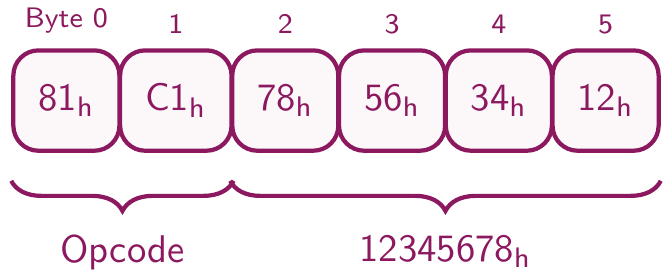
\includegraphics[width=0.1\textwidth]{opcode.png}

\section{Numbers}
\begin{description}
    \item[db] Byte, 8 Bit
    \item[dw] Word, 2 Byte, 16 Bit
    \item[dd] Doubleword, 4 Byte, 32 Bit
    \item[dq] Quadword, 8 Byte, 64 Bit
    \item [Double Quadword] 16 Byte, 128 Bit
\end{description}

\section{Byte Order}
Stellen innerhalb Bytes werden nicht vertauscht!
\begin{description}
    \item[Big-Endian] CA | FE
    \item[Little-Endian] FE | CA
\end{description}

\begin{lstlisting}[language={[x86masm]Assembler}]
text_length: dq after_my_text - my_text
my_text: db 'BSys 1'
after_my_text:
\end{lstlisting}

\section{Memory}
\begin{lstlisting}[language={[x86masm]Assembler}]
mov rax, [0x8000] ; move 8000h into rax
mov [0x8000], rax ; move val at rax into 0x8000
; move rbx into rax, no memory access:
mov rax, rbx
; error can't move memory to memory:
mov [0x8000], [0x7000]
\end{lstlisting}

\section{Einführung und Modulübersicht}
Ein Computer besteht aus Prozessoren, Hauptspeicher und Ein- und Ausgabegeräten. Das Betriebssystem verwaltet diese Ressourcen.

BILD: Grundmodell eines Computers

FMC-Modeling: Ecking - Aktiv, Rund - Passiv

Literatur:
\begin{itemize}
    \item Glatz, Betriebssysteme, 3. Auflage
    \item Tanenbaum, Modern Operating Systems, 4th Edition
    \item Silberschatz, Operating Systems, 9th Edition
    \item NASM Docs, C-Teil von cppreference.com
\end{itemize}

\section{Prozessor}
Merkvarianten-Analogie: Gedächtnis für wichtige Informationen, Papier für weniger wichtige Informationen. Gehirn ist eine kostbare Ressource, Papier ist preiswerter. Gleich ist dies mit dem Prozessor (Gedächtnis) und Speicher (Papier).

Kommunikationsprotokoll (Beispiel mit fenstern)

Speicherzellen sind nicht direkt an den Prozessor angebunden, es werden Adressen verwendet. Konzeptionell befindet sich ein Speicherbus dazwischen. Der Prozessor kennt nur den Bus. Dieser besteht aus Adressbus (unidirektional vom Prozessor aus), Datenbus (bidirektional, lesen/schreiben) und Steuersignalen (unidirektional vom Prozessor aus).

\subsection{Lesen/Schreiben}
SIEHE FOLIE 14

"Der Prozessor kann nur über den Speicherbus mit seiner Umwelt interagieren."

"Register sind nicht im Hauptspeicher, sondern innerhalb des Prozessors."

\begin{description}
    \item[Register]
    \item[Operation]
    \item[Instruction Pointer]
\end{description}

SEQUENZEN VON INSTRUKTIONEN SIEHE FOLIE 22

"Instruktionen sind von Hersteller zu Hersteller unterschiedlich. Die Gesamtheit aller Instruktionen eines Prozessors ist sein Maschinencode."

Prozessor-Zyklus (Abstraktion) FOLIE 27

    \section{Assembler}
    \subsection{Maschinencode}
    Prozessor arbeitet auf Bitebene. Intel 64 - Little Endian - 64 bit

    Intel Terms:
    \begin{description}
        \item[Byte] 8 bit
        \item[Word] 16 bit / 2 Byte
        \item[Doubleword] 32 bit / 4 Byte
        \item[Quadword] 64 bit / 8 Byte
        \item[Double Quadword] 128 bit / 16 Byte
    \end{description}

    Kleinste Einheit eines Intel-Prozessors: 8 Bit (1 Byte) - Ein Register (64 Bit) braucht also immer 8 Adressen. Ein einzelnes Bit lässt sich nicht adressieren!

    Byte Order:

    \subsection{Assembler}
    \begin{description}
        \item[Assembler] "Zusammensetzer" Übersetzer in Maschinencode
        \item[Assembly] die Sprache
        \item[db] DataByte: Zahl in Output schreiben (z.B. db 48 / db 0x35 / db 'Hello')
        \item[dw, dd, dq] Word, DWord, QWord
        \item[nop] 90h
    \end{description}

    \subsection{Referenzen in Assembler}
    Auf eine andere Stelle im Text verweisen.

    \subsection{Ausgabedateien}
    Flat-Form Binaries (plain, pure, raw), Wir brauchen aber Objekt-Dateien (Byte-Sequenz mit Zusatzinformationen, z.B. Symboltabelle/Labels)

    \section{Variablen}
    \subsection{Intel64 Register}
    \begin{description}
        \item[RAX] Accumulator, für einige Rechenoperationen das einzig mögliche Register
        \item[RCX] Counter für Schleifen und Stringoperationen
        \item[RDX] Pointer für I/O-Operationen
        \item[RBX] Datenpointer
        \item[RSI, RDI] Quell- (Source) und Zielindizes (Destination) für Stringoperationen
        \item[RSP] Stackpointer, Adresse des allozierten Stacks
        \item[RBP] Basepointer, Adresse innerhalb des Stacks, Basis des Rahmens der Funktion
        \item[R8-R15] Zusätzliche Register
    \end{description}

    \begin{tabular}{llllll}
      Nr. & 63..0 & 31..0 & 15..0 & 15..8 & 7..0\\
      \hline
      0 & RAX & EAX & AX & AH & AL\\
      1 & RCX & ECX & CX & CH & CL\\
      2 & RDX & EDX & DX & DH & DL\\
      3 & RBX & EBX & BX & BH & BL\\
      \hline
      4 & RSP & ESP & BP & - & SPL\\
      5 & RBP & EBP & BP & - & BPL\\
      6 & RSI & ESI & SI & - & SIL\\
      7 & RDI & EDI & DI & - & DIL\\
      \hline
      8 & R8 & R8D & R8W & - & R8L\\
      .. & .. & .. & .. & - & ..\\
      15 & R15 & R15D & R15W & - & R15L
    \end{tabular}

    Move-Operation (mov)
    \begin{description}
        \item[mov rax, rbx] Setze Inhalt von rax gleich rbx
        \item[mov rax, 0x8000] Setze Inhalt von rax gleich 8000h
        \item[mov rax, [0x8000]] Setze inhalt von rax gleich Inhalt von 8000h \dots 8007h
    \end{description}

    Assembler leitet den richtigen maschinencode aus der grösse des Registers ab.

    \section{C Toolchain}
    \begin{description}
        \item[C Präprozessor] verarbeitet C-Quelle, z.B. \texttt{includes}. Durchlauf 1: Kommentare entfernen, multi-liner to oneline. Durchlauf 2: Tokenization (Bezeichner (beginnt mit Buchstaben oder \_, gefolgt von Zeugs), Prärozessor-Zahlen (beginnt mit einer Ziffer, gefolgt von Ziffern, Buchstaben, \_ oder Exponenten), String- und Character-Literale (Anführungs und Schullzeichen von Strings), Operatoren und Satzzeichen (Greedy), Sonstige), Whitespace trennt tokens. Durchlauf 3: Präprozessod-Direktiven (z.B. \texttt{includes}, prepend mit hashtag) ausführen, Makros durch Expansion ersetzen (Objektartige (ohne Parameter) und Funktionsartige Makros, textersetzung, welche auch witzige formen z.B. int x = XYZ annehmen kann, aber nicht Rekursiv)
        \item[C Compiler] verarbeitet bereinigte C-Quelle (a.k.a \emph{Translation Unit}) (übersetzt \emph{eine} bereinige C-Datei in \emph{eine} Assembler-Datei, die bereinigte C-Datei enthält nur gültige C-Ausdrücke)
        \item[C Translation Unit] Folge von Deklarationen und Definitionen
        \item[Deklaration] Verknüpft einen Bezeichner Compiler-Intern mit einem Typen.
        \item[Definition] Umfasst auch immer eine Deklaration, legt aber auch den entsprechenden Speicher an.
        \item[Globale Variablen]
        \item[static] "Antiglobal"
        \item[Assembler] verarbeitet Assembler-Datei
        \item[Linker] verarbeitet Objektdateien zu Executables (viele Fehler)
    \end{description}

    \subsection{Includes}
    \texttt{<stdio.h>} sucht nur in den Systemverzeichnissen, \texttt{"stdio.h"} sucht erst im aktuellen Verzeichnis und dann in den anderen. Wenn vom Präprozessor gefunden, werden die drei Schritte des Präprozessors auch darauf ausgeführt (Farhad: Aufruf Rekursiv?)

\end{multicols*}
\end{document}
